\documentclass[a4paper,12pt]{article}
\usepackage[english,ukrainian,russian]{babel}
%\pagestyle{empty}
\linespread{1}
\usepackage{ucs}
\usepackage[utf8]{inputenc}
\usepackage[T2A]{fontenc}
\usepackage[paper=portrait,pagesize]{typearea}
\usepackage{amsmath}
\usepackage{bigints}
\usepackage{amsfonts}
\usepackage{graphicx}
\usepackage{amssymb}
\usepackage{cancel}
\usepackage{gensymb}
\usepackage{multirow}
\usepackage{rotate} 
\usepackage{pdflscape}
\usepackage{bigstrut}
\usepackage[pageanchor]{hyperref}
\usepackage{svg}
\usepackage{chngpage}
\newcommand{\dx}{\textbf{d}x}
\newcommand{\dt}{\textbf{d}t}
\newcommand{\du}{\textbf{d}u}
\newcommand{\dv}{\textbf{d}v}
\newcommand{\dy}{\textbf{d}y}
\newcommand{\ds}{\textbf{d}s}
\newcommand{\dz}{\textbf{d}z}
\newcommand{\arch}{\textrm{arcch}}
\newcommand{\arsh}{\textrm{arcsh}}
\newcommand{\dint}{\displaystyle\int}
\newcommand\tab[1][1cm]{\hspace*{#1}}
\newcommand{\dsum}{\displaystyle\sum}
\usepackage[left=20mm, top=20mm, right=15mm, bottom=15mm, nohead, nofoot]{geometry}
\newcommand{\ri}{R_i}
\newcommand{\re}{R_e}
\newcommand{\uo}{U_0}
\newcommand{\ik}{I_{kz}}
\newcommand{\po}{P_0}
\newcommand{\pio}{P_i}
\newcommand{\pe}{P_e}


\begin{document}
	\begin{center}
		\hfill \break
		\large{\textbf{НАЦIОНАЛЬНИЙ ТЕХНIЧНИЙ УНIВЕРСИТЕТ УКРАЇНИ\\
			«КИЇВСЬКИЙ ПОЛIТЕХНIЧНИЙ IНСТИТУТ»\\
			ФIЗИКО-ТЕХНIЧНИЙ IНСТИТУТ}}\\
		\hfill \break \hfill \break \hfill\break \hfill \break \hfill \break \hfill \break \hfill \break
		\hfill \break \hfill \break
		\large{Лабораторна робота с фізики №1}
		\begin{center}
			\normalsize{\textbf{ВНУТРIШНIЙ ОПIР ДЖЕРЕЛ ЕЛЕКТРИЧНОЇ ЕНЕРГIЇ ТА УЗГОДЖЕННЯ ПОТУЖНОСТЕЙ}}
		\end{center}
	\end{center}
	\hfill \break \hfill \break \hfill \break \hfill \break \hfill \break \hfill \break \hfill \break
	\hfill \break \hfill \break \hfill \break \hfill \break \hfill \break \hfill \break 
	\begin{flushright}
		\large{ \hspace{35pt} Виконав:\\
		студент групи ФI-12\\
		Завалій Олександр} 
	\end{flushright}
	\hfill \break \hfill \break \hfill \break \hfill \break \hfill \break \hfill \break \hfill \break
	\hfill \break \hfill \break 
	\begin{center} \textbf{Київ-2022} \end{center}
	\thispagestyle{empty} % выключаем отображение номера для этой страницы
	
\newpage
	\begin{center}
		\section* {РОЗДІЛ ПЕРШИЙ\\ТЕОРЕТИЧНА ДОВІДКА }
	\end{center}
	\textit{\textbf{Ключові поняття:} джерело струму або напруги, електрорушійна сила, ЕРС, вихідна напруга, напруга на клемах джерела, холостий хід, робота без навантаження, коротке замикання, закон Ома, закони Кірхгофа, режими узгодження. }
	
	\begin{center}
		\textbf{Мета роботи}
	\end{center}
	\begin{enumerate}
		\item Дослідити закон Ома для ділянки та всього кола.  
		\item Визначити внутрішній опір джерел електричної енергії.  
		\item Дослідити узгодження потужностей джерела та споживача.  
		\item Визначити, до якої групи відноситься те чи інше джерело за величиною внутрішнього опору – до джерел напруги або джерел струму.  
		\item Визначити за якого режиму джерело буде віддавати максимальну корисну потужність та матиме максимальний ККД. 
	\end{enumerate}
	
	\begin{center}
		\textbf{Теоретичне підгрунтя }
	\end{center}
	Розглянемо електричне коло (рис.1), яке складається з джерела електричної енергії зі своїм внутрішнім опором $R_i$ та зовнішнім опором $R_e$ – змінним опором навантаження. Струм в такому колі визначається за законом Ома рівнянням:\\
	$$I=\dfrac{U_0}{R_i+R_e}\eqno(1)$$
	Ми отримаємо найменше значення $I=0$ якщо $R_e=\infty$, та найбільше $I=I_{max}$, якщо $R_e=0$.
	Із всіх режимів роботи електричних кіл та елементів навантаження найхарактернішими є:
	\begin{enumerate}
		\item[-] Режим кола, коли опір навантаження $R_e=\infty$ визначається як режим холостого ходу, струм не протікає в колі, тому не має падіння напруги на $R_i$. Тобто на клемах джерела присутня напруга холостого ходу $U_0$. 
		\item[-] Режим кола, коли $\re=0$ визначається як режим короткого замикання, струм в колі максимальний і визначається як $\ik=\dfrac{\uo}{\ri}$
		\item[-] Режим за $\re=\ri$ – узгодження потужності (або узгодження опорів). 
	\end{enumerate}
	\begin{figure}[!h]
		\begin{center}
			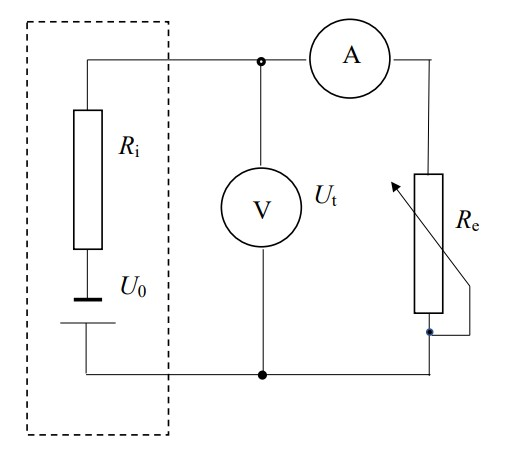
\includegraphics[scale=0.5]{Prt sc/Shema.jpg}
		\end{center}
		\caption{Схема вимірювання вихідної напруги та струму, штриховою лінією позначено джерело енергії, в якому окремо виділено внутрішній опір.}
		\label{1}
	\end{figure}

\newpage
	Прослідкуємо як змінюються спад напруги на опорах $\ri$ та $\re$ в залежності від струму в колі. Спад напруги на внутрішньому опорі дорівнює:\\
	$$U_{\ri}=I\ri\eqno(2)$$
	
	Величина цього спаду пропорційна величині струму і змінюється від нуля до найбільшого значення. 
	Спад напруги на зовнішньому опорі навантаження $\re$ згідно другого правила Кірхгофа, дорівнює: 
	$$U_{\re}=\uo-U_{\ri}\eqno(3)$$
	
	Цей спад напруги також знаходиться в лінійній залежності від струму. Так як опір навантаження під’єднаний до вихідних клем джерела, то спад напруги на опорі навантаження можна вважати як вихідну напругу джерела яка визначається за рівнянням: 
	$$U_t=U_0-IR_i\eqno(4)$$
	
	Нормовані графіки, які показують залежність $U_{\ri}$ та $U_{\re}$ від струму $I$ наведені \\на рис. 2.
	\begin{figure}[!h]
		\begin{center}
			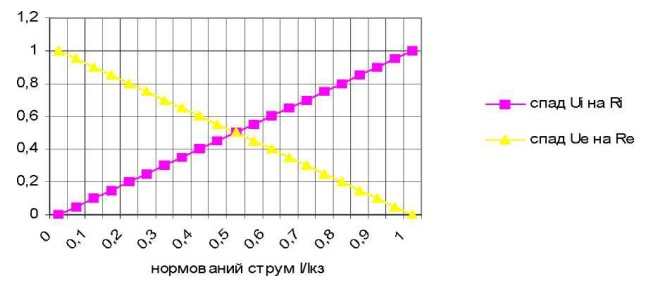
\includegraphics[scale=0.5]{Prt sc/Shema_2.jpg}
		\end{center}
		\caption{Нормовані залежності спадів напруг від струму на внутрішньому і зовнішньому опорах.}
		\label{2}
	\end{figure}
	
\newpage
	За умови $\ri-\re$ їхня сума дорівнюватиме $2R$, має місце співвідношення:
	$$I=\dfrac{\uo}{2R}=\dfrac{\ik}{2}\eqno(5)$$
	
	І спад напруг на опорах рівні між собою, тобто: 
	$$U_{\ri}=U_{\re}=\dfrac{\uo}{2}\eqno(6)$$
	
	Такий режим називається, як було вище вказано, режимом узгодження внутрішнього опору джерела та опору споживача. 
	
	Визначимо співвідношення між потужностями, які виділяються на елементах електричного кола. Повна потужність електричного кола визначається за співвідношенням:
	$$\po=\uo\ik\eqno(7)$$
	
	Повна потужність джерела складається з потужності, яка виділяється на внутрішньому опорі джерела i визначається за співвідношенням:
	$$\pio=I^2\ri\eqno(8)$$
	
	і змінюється пропорційно квадрату струму. Потужність, яка виділяється на опорі навантаження $\re$
	$$\pe=I^2\re\eqno(9)$$
	
	Визначається як різниця між повною потужністю $P$ та потужністю, яка виділяється на внутрішньому опорі $\ri$, тобто 
	$$\pe=\po-\pio=\uo-I^2\ri\eqno(10)$$
	
	Потужність $\pe$ дорівнює нулю, коли струм за $I=I_{xx}=0,\: \pe(I)=\uo-2I\ri=0$
	
	Для визначення найбільшого значення потужності візьмемо першу похідну від минулої формули та прирівняємо її до 0. Звідти отримаємо співвідношення: 
	$$\uo=2I\ri\eqno(11)$$
	
	Але при будь-якому значенні опору $\re$ (у будь-якому режимі) згідно 2 правила Кірхгофа: 
	$$\uo=I\ri+I\re\eqno(12)$$
	
	Порівнюючи два останні вирази видно, що потужність $\pe$ досягає найбільшого значення при $\re=\ri$, коли струм в колі буде відповідати співвідношенням: 
	$$I=\dfrac{\uo}{2\ri}=\dfrac{\ik}{2}\eqno(13)$$
	
	Тобто максимальна потужність $\pe$, яка виділяється на зовнішньому опорі навантаження, буде дорівнювати потужності 
	$\pio$, яка виділяється на внутрішньому опорі і буде дорівнювати $\dfrac{1}{4}\po$
	– режим узгодження потужностей джерела та споживача:
	$$\pe=I^2\re=\dfrac{\uo^2\ri^2}{4\ri^2}=\dfrac{\uo\ik}{4}\eqno(14)$$

\newpage
	Графіки, які виявляють залежність потужностей $P,\: \pi,\: \pe$ від струму наведені на рис. 3.
	\begin{figure}[!h]
		\begin{center}
			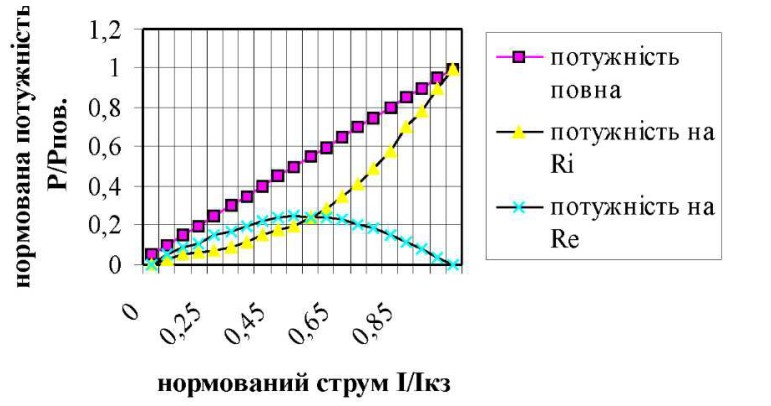
\includegraphics[scale=0.5]{Prt sc/Shema_3.jpg}
		\end{center}
		\caption{Нормована залежність зміни потужностей від струму.}
		\label{3}
	\end{figure}\\
	А залежність потужності від співвідношення опорів – на рис. 4.\\
	\begin{figure}[h]
		\begin{center}
			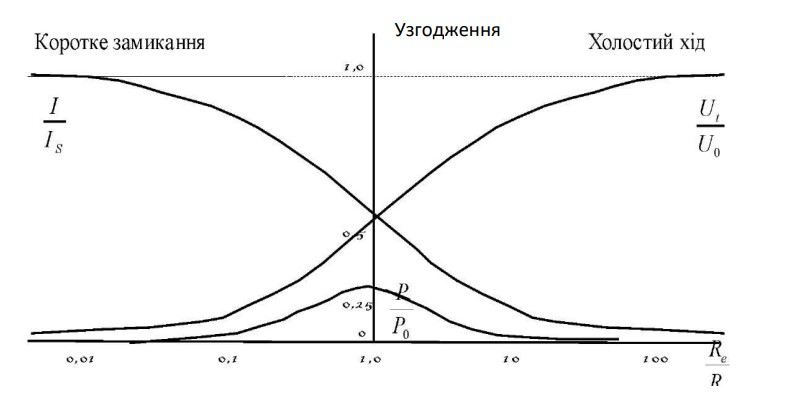
\includegraphics[scale=0.5]{Prt sc/Shema_4.jpg}
		\end{center}
		\caption{Нормовані графіки залежності потужності джерела від навантаження (відношення опору навантаження до внутрішнього опору джерела).}
		\label{4}
	\end{figure}
	
	З’ясуємо які режими роботи джерела електричної енергії найбільш доцільні: 
	\begin{enumerate}
		\item[-] За яких умов джерело розвине максимальну корисну потужність.
		\item[-] За якого режиму джерело матиме найбільший $KKD-\eta$
	\end{enumerate}
	Корисна потужність в електричному колі – це потужність $\pe$, яка виділяється на 
	опорі навантаження $\re$. Потужність, яка виділяється на внутрішньому опорі $\ri$, це 
	потужність втрат $\pio$. Режим, коли джерело розвиває найбільшу корисну потужність, має місце при $\re=\ri$, в цьому випадку струм в колі $\i=\dfrac{\ik}{2}$, а корисна 
	потужність і однакова з нею потужність втрат дорівнює:
	$$\pio=\pe=\dfrac{\uo\ik}{2}\eqno(15)$$

\newpage
	Максимальна потужність, яку може розвинути джерело: 
	$$P=\pio+\pe=\uo\ik\eqno(16)$$
	
	KKD – коефіцієнт корисної дії дорівнюватиме:
	$$\eta=\dfrac{\pe}{\po}$$
	
	Окрім розглянених режимів найбільш широко використовуваним є номінальний режим роботи. Це такий режим для якого розраховане джерело електричної енергії або електроприймач. Для електричних величин, що визначають 
	номінальний режим, відносяться номінальна напруга, номінальний струм, номінальна потужність. Генератори, електроприймачі та інші елементи електричних установок виробляють не на будь–які напруги, а на обмежене число визначених напруг
	
	\textbf{Джерело напруги} – джерело енергії, підтримує напругу на клемах, величина якої якого не залежить від опору навантаження, а внутрішній опір набагато менший за опір навантаження $\ri<<\re$, зокрема за максимальне значення опору навантаження (наприклад, батареї, акумулятори, мережа).
	
	\textbf{Джерело струму} – джерело енергії, струм якого не залежить від опору навантаження, а внутрішній опір набагато більший за опір навантаження $\ri>>\re$, зокрема за мінімальне значення опору навантаження (транзистори, котушки індуктивності). 
	
	\begin{center}
		\textbf{Експериментальне обладнання: }
	\end{center}
	Експериментальне обладнання складається з:
	\begin{enumerate}
		\item Трьох джерел електричної енергії:
			\begin{enumerate}
				\item[-] Батарейка з трьох марганцево-цинкових елементів для кишенькових ліхтариків;
				\item[-] Свинцевого кислого акумулятора; 
				\item[-] Електронного блока живлення; 
			\end{enumerate} 
		\item Реостатів з максимальним опором 10 Ом, 45 Ом, 100 Ом. 
		\item Магнітоелектричного мультиметра.
		\item Цифрового мультиметра.  
	\end{enumerate}
	В якості амперметра використовується магнітоелектричний мультиметр. Як вольтметр – цифровий мультиметр. 

\newpage
	\begin{center}
		\section* {РОЗДІЛ ДРУГИЙ\\Теоретичні основи експерименту}
	\end{center}
	\textbf{Дослід №1 }
	\begin{enumerate}
		\item Зберіть вимірювальну схему згідно рис.1 (в якості джерела використайте марганцево-цинкову батарейку для кишенькового ліхтарика) 
		\item В якості навантаження використати реостат з максимальним опором 45 або 100 Ом. 
		\item Виміряти напругу холостого ходу – $\uo$ (на клемах джерела без навантаження) 
		\item За допомогою вольтметра виміряти залежності напруги $U_{\re}$ на опорі навантаження від струму $I$, тобто від величини опору навантаження (струм змінювати реостат з кроком 0.1А до максимального значення 2А, тобто зробити 15-20 вимірів). 
		\item Встановіть опір навантаження таким, щоб спад напруги на опорі навантаження $U_{\re}$
		становить $\dfrac{1}{2}\uo$. В цьому випадку опір навантаження буде дорівнювати внутрішньому опору джерела $\re=\ri$ (режим узгодження опорів або потужностей). Не змінюючи положення реостата за допомогою омметра виміряйте опір навантаження. 
		\item Отримані дані занесіть до таблиці. 
	\end{enumerate}
	\textbf{Дослід №2} 
	\begin{enumerate}
		\item Зберіть вимірювальну схему згідно рис.1 (в якості джерела використайте свинцевий акумулятор)  
		\item В якості навантаження використати реостат з максимальним опором 45 або 100 Ом. 
		\item Виміряти напругу холостого ходу – $\uo$ (на клемах джерела без навантаження). 
		\item Виміряти залежності напруги $U+{\re}$ від струму $I$, тобто від величини о навантаження (струм змінювати). 
		\item Отримані дані занесіть до таблиці. 
	\end{enumerate}
	\textbf{Дослід №3} 
	\begin{enumerate}
		\item Зберіть вимірювальну схему згідно рис.1(в якості джерела використайте блок живлення, який живиться від силової мережі). 
		\item В якості навантаження використати реостат з максимальним опором 45 або 100 Ом. 
		\item Виміряти напругу холостого ходу – $\uo$ (на клемах джерела без навантаження). 
		\item За допомогою вольтметра для кожного значення струму виміряйте залежність спаду напруги на опорі навантаження $U+{\re}$ від струму $I$, тобто від величини опору навантаження (струм змінювати реостат з кроком 0,1А до максимального значення 2А, тобто зробити 15-20 вимірів) 
		\item Отримані дані занесіть до таблиці. 
	\end{enumerate}

\newpage
	\begin{center}
		\textbf{Завдання}
	\end{center}
	\begin{enumerate}
		\item Побудуйте графік залежності $U(I)$ для всіх досліджуваних джерел. Зробіть аппроксимацию для кожного побудованого графіка. 
		\item За апроксимацією графіків визначте внутрішній опір кожного джерела за різних режимів навантаження. 
		\item Побудуйте нормовані графіки залежності потужності від струму аналогічно рис.3 та рис.4 
		\item Визначте похибки, поясніть за яких факторів виникли ці похибки. 
		\item Зробіть відповідні висновки. 
		\item На підставі проведених дослідів та розрахунків дайте остаточну характеристику кожного з джерел (джерела струму та джерела напруги). 
		\item Визначте за яких умов джерело може бути джерелом напруги чи джерелом струму. 
	\end{enumerate}
	
\newpage
	\begin{center}
		\section* {РОЗДІЛ ТРЕТІЙ\\Експериментальні дані}
	\end{center}
	
	\begin{figure}[h!]
		\begin{minipage}[h]{0.5\linewidth}
			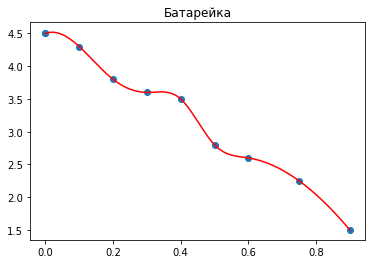
\includegraphics[width=1\linewidth]{Prt sc/Figure_1_1.jpeg}
			\label{Figure_1_1}
			\caption{Графiк залежності $U$ вiд $I$.}
		\end{minipage}
		\begin{minipage}[h]{0.5\linewidth}
			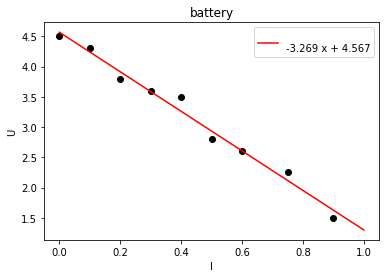
\includegraphics[width=1\linewidth]{Prt sc/Figure_1_2.jpeg}
			\label{Figure_1_2}
			\caption{Апроксимований графiк залежності $U$ вiд $I$.}
		\end{minipage}
	\end{figure}
	
	\begin{figure}[h!]
		\begin{minipage}[h]{0.5\linewidth}
			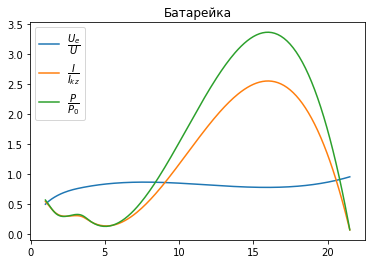
\includegraphics[width=1\linewidth]{Prt sc/Figure_1_3.jpeg}
			\caption{Нормований графiк залежностi потужностi джерела вiд навантаження}
		\end{minipage}
		\begin{minipage}[h]{0.5\linewidth}
			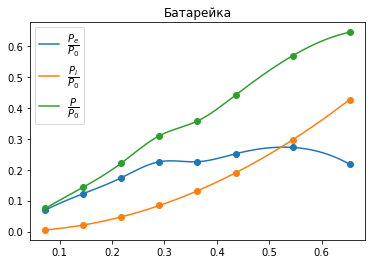
\includegraphics[width=1\linewidth]{Prt sc/Figure_1_4.jpeg}
			\caption{Нормована залежність змiни потужностей вiд струму.}
		\end{minipage}
	\end{figure}
	
	\begin{flushleft}
		\textbf{Внутрішній опір}
	\end{flushleft}
	З графiку бачимо, що лiнiйна апроксимацiя залежностi $U$ вiд $I$ батарейки має вигляд:\\ $$y=-3.329x+4.604$$
	А отже $\ri$ апроксимоване дорiвнює $3.329$
	
\newpage
	\begin{figure}[h]
		\centering
		\begin{minipage}[h]{0.5\linewidth}
			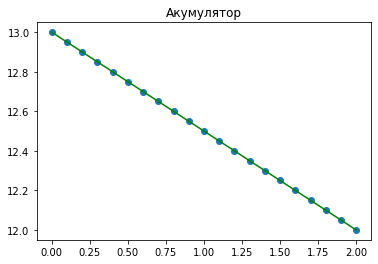
\includegraphics[width=1\linewidth]{Prt sc/Figure_2_1.jpeg}  
		\end{minipage}
		\caption{Графiк залежності $U$ вiд $I$.}
	\end{figure}
	\begin{figure}[h]
		\centering
		\begin{minipage}[h]{0.5\linewidth}
			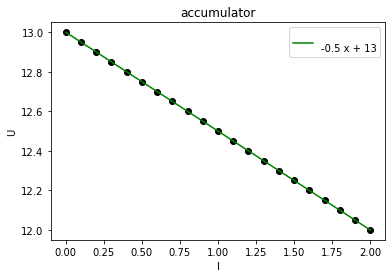
\includegraphics[width=1\linewidth]{Prt sc/Figure_2_2.jpeg} \begin{center}(b)\end{center}
		\end{minipage}
		\caption{Апроксимований графiк залежності $U$ вiд $I$.}
	\end{figure}
	
	\begin{flushleft}
		\textbf{Внутрішній опір}
	\end{flushleft}
	З графiку бачимо, що лiнiйна апроксимацiя залежностi $U$ вiд $I$ акумулятора має вигляд:\\ $$y=-0.5x+13$$
	А отже $\ri$ апроксимоване дорiвнює $0.5$
	
\newpage
	\begin{figure}[h]
		\centering
		\begin{minipage}[h]{0.5\linewidth}
			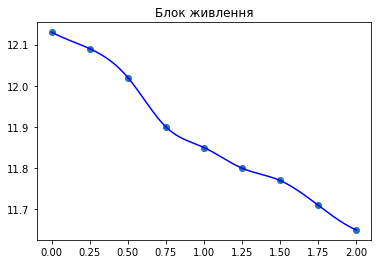
\includegraphics[width=1\linewidth]{Prt sc/Figure_3_1.jpeg} \caption{Графiк залежності $U$ вiд $I$.} 
		\end{minipage}
	\end{figure}
	\begin{figure}[h]
		\centering
		\begin{minipage}[h]{0.5\linewidth}
			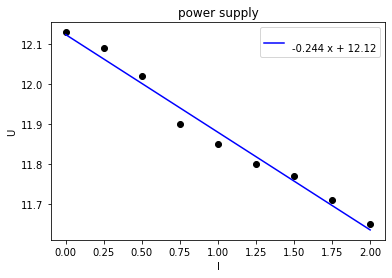
\includegraphics[width=1\linewidth]{Prt sc/Figure_3_2.jpeg}
		\end{minipage}
		\caption{Апроксимований графiк залежності $U$ вiд $I$.}
	\end{figure}
	
	\begin{flushleft}
		\textbf{Внутрішній опір}
	\end{flushleft}
	З графiку бачимо, що лiнiйна апроксимацiя залежностi $U$ вiд $I$ блоку живлення має вигляд:\\ $$y=-0.2414x+12.12$$
	А отже $\ri$ апроксимоване дорiвнює $0.2414$
	
\newpage
	\subsection*{Обчислення}
	Для різних джерел струму (акумулятора, блоку живлення та батарейки) було знято покази сили струму та напруги длявивчення залежності $U(I)$.Для визначення силових діаграм залежностей між напругою на клемах та силою струму було побудовано відповідні рівняння прямих $y=kx+b$ де $x$–сила струму, $y$–напруга, а коефіцієнти $k$ та $b$ знаходяться за відповідними формулами:
	$$k=\dfrac{<IU>-<I><U>}{<I^2>-<I>^2};\: b=<U>-k<I>$$
	Отримані дані занесено до таблиць 4-9.\\
	\begin{center}
		\textbf{Похибки.}
	\end{center}
	Формула для обчислення похибок:
	$$\langle\ri\rangle=\dfrac{1}{n}\sum_{k=1}^{n}R_{ik}\eqno(1)$$
	$$\Delta\ri=\sqrt{(\Delta R_{r})^2+(\Delta R_{s})^2},\: R_r=\sqrt{\dfrac{\sum\limits_{k=1}^{n}(R_{ik}-\ri)^2}{n^2-n}}\eqno(2)$$
	$$\varepsilon\ri=\dfrac{\Delta\ri}{\ri}\eqno(3)$$
	$$\ri=\dfrac{R_{i_1}+R_{i_2}+...+R_{i_n}}{n}$$
	Підставляючи відповідні значення у відповідні формули отримаємо такі результати:
	\begin{table}[h!]
		\centering
		\begin{tabular}{|l|c|}
			\hline
			Батарейка     & $\langle\ri\rangle=2.99$ \\ \hline
			Акумулятор    & $\langle\ri\rangle=0.5$ \\ \hline
			Блок живлення & $\langle\ri\rangle=0.24$ \\ \hline
		\end{tabular}
	\end{table}
	\begin{table}[h!]
		\centering
		\begin{tabular}{|l|c|}
			\hline
			Батарейка     & $\Delta\ri=17.92\%$ \\ \hline
			Акумулятор    & $\Delta\ri=0\%$  \\ \hline
			Блок живлення & $\Delta\ri=1.54\%$ \\ \hline
		\end{tabular}
	\end{table}
	\begin{table}[h!]
		\centering
		\begin{tabular}{|l|c|}
			\hline
			Батарейка     & $\varepsilon\ri=6\%$ \\ \hline
			Акумулятор    & $\varepsilon\ri=0\%$  \\ \hline
			Блок живлення & $\varepsilon\ri=6.32\%$ \\ \hline
		\end{tabular}
	\end{table}
	Похибки з'являються через неточність вимірів. За відсутністю систематичної похибки $(R_r)$ можна дійти висновку, що це теж вплинуло на результат обчислень.
	
\newpage
	\begin{center}
		\section* {РОЗДІЛ ЧЕТВЕРТИЙ\\Висновки}
	\end{center}
	В ході виконання лабораторної роботи дослідив узгодження потужностей джерела та споживача, визначив режим роботи за якого джерело буде віддавати максимальну корисну потужність та матиме при цьому максимальне ККД. Метою ЛР було ознайомлення з такими поняттями: закон Ома, опір, сила струму, напруга, потужність, ККД в електричному полi. 
	
	Пiсля обробки даних та необхiдних пiдрахункiв було визначено залежностi напруг на клемах джерел струму вiд сили струму. Всього побудував три залежностi: для батарейки, акумулятора та блоку живлення.
	
	З графіків типу (a) на сторінка 9, 10 та 11 можна спостерігати лінійну залежність напруги від сили струму. Хочу зазначити, що експериментальні залежності можуть суттєво від них відрізнятись тобто вони мають криволінійну залежність. В нашому випадку такий характер залежності означає, що внутрішні опори $\ri$ джерел струму є сталими. 
	
	З графіків типу (с) на сторінка 9, 10 та 11 бачимо, що нормовані залежності напруги та струму від зовнішнього навантаження є взаємно-протилежними, що цілком відповідає дійсності. Максимум потужності можна спостерігати за умови узгодженості потужностей. \\
	
	\begin{center}
		\textbf{За результатами обробки дослідних даних отримано:}
	\end{center}
	Внутрішній опір джерела напруги обчислюємо за формулою $\ri=\dfrac{\uo}{\ik}$:
	\begin{enumerate}
		\item[-] Батарейка: $\ri=\dfrac{4.5}{1.352}=3.329$ Ом, $\uo$ = 4.5 В.
		\item[-] Акумулятор: $\ri=\dfrac{13}{26}=0.5$ Ом, $\uo$ = 13 В.
		\item[-] Блок живлення: $\ri=\dfrac{12.13}{50.243}=0.241$ Ом, $\uo$ = 12.13 В.
	\end{enumerate}

	\KOMAoptions{paper=A3,paper=landscape,DIV=20,pagesize}
	\begin{center}
		\subsection*{\LARGE{Таблиці}}
	\end{center}
	\begin{table}[htbp]
		\centering
		\caption{Батарейка}
		\begin{tabular}{|c|c|c|c|c|c|c|c|c|c|c|c|c|c|c|c|c|c|c|c|}
			\hline
			\textbf{$U_0, B$}    & \textbf{$I, A$} & \textbf{$U, B$} & \textbf{$R_i(approx), Om$} & \textbf{$R_i, Om$} & \textbf{$R_e, Om$} & \textbf{$U_i, B$} & \textbf{$U_e, B$} & \textbf{$P_e$, Вт} & \textbf{$P_i$, Вт} & \textbf{$\ik, A$}     & \textbf{$P_0$, Вт}     & \textbf{$P_e/P_0$} & \textbf{$P_i/P_0$} & \textbf{$P$, Вт} & \textbf{$P/P_0$} & \textbf{KKD, \%} & \textbf{${\langle R\rangle}, Om$}     & \textbf{$\Delta R, Om$} & \textbf{$\varepsilon R, Om$} \\ \hline
			\multirow{8}{*}{4.5} & 0.1        & 4.3        & \multirow{8}{*}{3.33} & 2.0           & 43.0          & 0.33          & 4.17          & 0.43          & 0.03          & \multirow{8}{*}{1.35} & \multirow{8}{*}{6.08} & 0.07               & 0.01               & 0.46       & 0.08            & 7.07                & \multirow{8}{*}{2.99} & \multirow{8}{*}{17.92} & \multirow{8}{*}{6.0} \\ \cline{2-3} \cline{5-10} \cline{13-17}
			& 0.2        & 3.8        &                       & 3.5           & 19.0          & 0.67          & 3.83          & 0.76          & 0.13          &                       &                       & 0.12               & 0.02               & 0.89       & 0.15            & 12.49               &                       &                        &                      \\ \cline{2-3} \cline{5-10} \cline{13-17}
			& 0.3        & 3.6        &                       & 3.0           & 12.0          & 1.0           & 3.5           & 1.08          & 0.3           &                       &                       & 0.18               & 0.05               & 1.38       & 0.23            & 17.75               &                       &                        &                      \\ \cline{2-3} \cline{5-10} \cline{13-17}
			& 0.4        & 3.5        &                       & 2.5           & 8.75          & 1.33          & 3.17          & 1.4           & 0.53          &                       &                       & 0.23               & 0.09               & 1.93       & 0.32            & 23.01               &                       &                        &                      \\ \cline{2-3} \cline{5-10} \cline{13-17}
			& 0.5        & 2.8        &                       & 3.4           & 5.6           & 1.66          & 2.84          & 1.4           & 0.83          &                       &                       & 0.23               & 0.14               & 2.23       & 0.37            & 23.01               &                       &                        &                      \\ \cline{2-3} \cline{5-10} \cline{13-17}
			& 0.6        & 2.6        &                       & 3.17          & 4.33          & 2.0           & 2.5           & 1.56          & 1.2           &                       &                       & 0.26               & 0.2                & 2.76       & 0.45            & 25.64               &                       &                        &                      \\ \cline{2-3} \cline{5-10} \cline{13-17}
			& 0.75       & 2.25       &                       & 3.0           & 3.0           & 2.5           & 2.0           & 1.69          & 1.87          &                       &                       & 0.28               & 0.31               & 3.56       & 0.59            & 27.74               &                       &                        &                      \\ \cline{2-3} \cline{5-10} \cline{13-17}
			& 0.9        & 1.5        &                       & 3.33          & 1.67          & 3.0           & 1.5           & 1.35          & 2.7           &                       &                       & 0.22               & 0.44               & 4.05       & 0.67            & 22.19               &                       &                        &                      \\ \hline
		\end{tabular}%
	\end{table}
	
	\begin{table}[htbp]
		\centering
		\caption{Акумулятор}
		\begin{tabular}{|c|c|c|c|c|c|c|c|c|c|c|c|c|c|c|c|c|c|c|c|}
			\hline
			\textbf{$U_0, B$}    & \textbf{$I, A$} & \textbf{$U, B$} & \textbf{$R_i(approx), Om$} & \textbf{$R_i, Om$} & \textbf{$R_e, Om$} & \textbf{$U_i, B$} & \textbf{$U_e, B$} & \textbf{$P_e$, Вт} & \textbf{$P_i$, Вт} & \textbf{$I_kz, A$}     & \textbf{$P_0, Вт$}      & \textbf{$P_e/P_0$} & \textbf{$P_i/P_0$} & \textbf{$P$, Вт} & \textbf{$P/P_0$} & \textbf{KKD, \%} & \textbf{${\langle R\rangle}, Om$}      & \textbf{$\Delta R, Om$} & \textbf{$\varepsilon R, Om$} \\ \hline
			\multirow{20}{*}{13} & 0.1        & 12.95      & \multirow{20}{*}{0.5} & 0.5           & 129.5         & 0.05          & 12.95         & 1.3           & 0.0           & \multirow{20}{*}{26.0} & \multirow{20}{*}{338.0} & 0.0                & 0.0                & 1.3        & 0.0             & 0.38                & \multirow{20}{*}{0.5} & \multirow{20}{*}{0.0} & \multirow{20}{*}{0.0} \\ \cline{2-3} \cline{5-10} \cline{13-17}
			& 0.2        & 12.9       &                       & 0.5           & 64.5          & 0.1           & 12.9          & 2.58          & 0.02          &                        &                         & 0.01               & 0.0                & 2.6        & 0.01            & 0.76                &                       &                       &                       \\ \cline{2-3} \cline{5-10} \cline{13-17}
			& 0.3        & 12.85      &                       & 0.5           & 42.83         & 0.15          & 12.85         & 3.86          & 0.04          &                        &                         & 0.01               & 0.0                & 3.9        & 0.01            & 1.14                &                       &                       &                       \\ \cline{2-3} \cline{5-10} \cline{13-17}
			& 0.4        & 12.8       &                       & 0.5           & 32.0          & 0.2           & 12.8          & 5.12          & 0.08          &                        &                         & 0.02               & 0.0                & 5.2        & 0.02            & 1.51                &                       &                       &                       \\ \cline{2-3} \cline{5-10} \cline{13-17}
			& 0.5        & 12.75      &                       & 0.5           & 25.5          & 0.25          & 12.75         & 6.38          & 0.12          &                        &                         & 0.02               & 0.0                & 6.5        & 0.02            & 1.89                &                       &                       &                       \\ \cline{2-3} \cline{5-10} \cline{13-17}
			& 0.6        & 12.7       &                       & 0.5           & 21.17         & 0.3           & 12.7          & 7.62          & 0.18          &                        &                         & 0.02               & 0.0                & 7.8        & 0.02            & 2.25                &                       &                       &                       \\ \cline{2-3} \cline{5-10} \cline{13-17}
			& 0.7        & 12.65      &                       & 0.5           & 18.07         & 0.35          & 12.65         & 8.86          & 0.24          &                        &                         & 0.03               & 0.0                & 9.1        & 0.03            & 2.62                &                       &                       &                       \\ \cline{2-3} \cline{5-10} \cline{13-17}
			& 0.8        & 12.6       &                       & 0.5           & 15.75         & 0.4           & 12.6          & 10.08         & 0.32          &                        &                         & 0.03               & 0.0                & 10.4       & 0.03            & 2.98                &                       &                       &                       \\ \cline{2-3} \cline{5-10} \cline{13-17}
			& 0.9        & 12.55      &                       & 0.5           & 13.94         & 0.45          & 12.55         & 11.3          & 0.4           &                        &                         & 0.03               & 0.0                & 11.7       & 0.03            & 3.34                &                       &                       &                       \\ \cline{2-3} \cline{5-10} \cline{13-17}
			& 1.0        & 12.5       &                       & 0.5           & 12.5          & 0.5           & 12.5          & 12.5          & 0.5           &                        &                         & 0.04               & 0.0                & 13.0       & 0.04            & 3.7                 &                       &                       &                       \\ \cline{2-3} \cline{5-10} \cline{13-17}
			& 1.1        & 12.45      &                       & 0.5           & 11.32         & 0.55          & 12.45         & 13.7          & 0.6           &                        &                         & 0.04               & 0.0                & 14.3       & 0.04            & 4.05                &                       &                       &                       \\ \cline{2-3} \cline{5-10} \cline{13-17}
			& 1.2        & 12.4       &                       & 0.5           & 10.33         & 0.6           & 12.4          & 14.88         & 0.72          &                        &                         & 0.04               & 0.0                & 15.6       & 0.05            & 4.4                 &                       &                       &                       \\ \cline{2-3} \cline{5-10} \cline{13-17}
			& 1.3        & 12.35      &                       & 0.5           & 9.5           & 0.65          & 12.35         & 16.06         & 0.84          &                        &                         & 0.05               & 0.0                & 16.9       & 0.05            & 4.75                &                       &                       &                       \\ \cline{2-3} \cline{5-10} \cline{13-17}
			& 1.4        & 12.3       &                       & 0.5           & 8.79          & 0.7           & 12.3          & 17.22         & 0.98          &                        &                         & 0.05               & 0.0                & 18.2       & 0.05            & 5.09                &                       &                       &                       \\ \cline{2-3} \cline{5-10} \cline{13-17}
			& 1.5        & 12.25      &                       & 0.5           & 8.17          & 0.75          & 12.25         & 18.38         & 1.12          &                        &                         & 0.05               & 0.0                & 19.5       & 0.06            & 5.44                &                       &                       &                       \\ \cline{2-3} \cline{5-10} \cline{13-17}
			& 1.6        & 12.2       &                       & 0.5           & 7.62          & 0.8           & 12.2          & 19.52         & 1.28          &                        &                         & 0.06               & 0.0                & 20.8       & 0.06            & 5.78                &                       &                       &                       \\ \cline{2-3} \cline{5-10} \cline{13-17}
			& 1.7        & 12.15      &                       & 0.5           & 7.15          & 0.85          & 12.15         & 20.65         & 1.44          &                        &                         & 0.06               & 0.0                & 22.1       & 0.07            & 6.11                &                       &                       &                       \\ \cline{2-3} \cline{5-10} \cline{13-17}
			& 1.8        & 12.1       &                       & 0.5           & 6.72          & 0.9           & 12.1          & 21.78         & 1.62          &                        &                         & 0.06               & 0.0                & 23.4       & 0.07            & 6.44                &                       &                       &                       \\ \cline{2-3} \cline{5-10} \cline{13-17}
			& 1.9        & 12.05      &                       & 0.5           & 6.34          & 0.95          & 12.05         & 22.9          & 1.8           &                        &                         & 0.07               & 0.01               & 24.7       & 0.07            & 6.77                &                       &                       &                       \\ \cline{2-3} \cline{5-10} \cline{13-17}
			& 2.0        & 12.0       &                       & 0.5           & 6.0           & 1.0           & 12.0          & 24.0          & 2.0           &                        &                         & 0.07               & 0.01               & 26.0       & 0.08            & 7.1                 &                       &                       &                       \\ \hline
		\end{tabular}%
	\end{table}

	$\po=\uo\ik=4.5\cdot1.352=6.084$\\
	$\po=\uo\ik=13\cdot26=338$\\
	$\po=\uo\ik=12.13\cdot50.243=609.443$\\

\newpage
	\KOMAoptions{paper=A3,paper=landscape,DIV=20,pagesize}
	\begin{table}[htbp]
		\centering
		\caption{Блок живлення}
		\begin{tabular}{|c|c|c|c|c|c|c|c|c|c|c|c|c|c|c|c|c|c|c|c|}
			\hline
			\textbf{$U_0, B$}      & \textbf{$I, A$} & \textbf{$U, B$} & \textbf{$R_i(approx), Om$} & \textbf{$R_i, Om$} & \textbf{$R_e, Om$} & \textbf{$U_i, B$} & \textbf{$U_e, B$} & \textbf{$P_e$, Вт} & \textbf{$P_i$, Вт} & \textbf{$I_kz, A$}      & \textbf{$P_0$, Вт}       & \textbf{$P_e/P_0$} & \textbf{$P_i/P_0$} & \textbf{$P$, Вт} & \textbf{$P/P_0$} & \textbf{KKD, \%} & \textbf{${\langle R\rangle}, Om$}     & \textbf{$\Delta R, Om$} & \textbf{$\varepsilon R, Om$} \\ \hline
			\multirow{8}{*}{12.13} & 0.25       & 12.09      & \multirow{8}{*}{0.24} & 0.16          & 48.36         & 0.06          & 12.07         & 3.02          & 0.02          & \multirow{8}{*}{50.24} & \multirow{8}{*}{609.44} & 0.0                & 0.0                & 3.04       & 0.0             & 0.5                 & \multirow{8}{*}{0.24} & \multirow{8}{*}{1.54} & \multirow{8}{*}{6.32} \\ \cline{2-3} \cline{5-10} \cline{13-17}
			& 0.5        & 12.02      &                       & 0.22          & 24.04         & 0.12          & 12.01         & 6.01          & 0.06          &                        &                         & 0.01               & 0.0                & 6.07       & 0.01            & 0.99                &                       &                       &                       \\ \cline{2-3} \cline{5-10} \cline{13-17}
			& 0.75       & 11.9       &                       & 0.31          & 15.87         & 0.18          & 11.95         & 8.93          & 0.14          &                        &                         & 0.01               & 0.0                & 9.06       & 0.01            & 1.46                &                       &                       &                       \\ \cline{2-3} \cline{5-10} \cline{13-17}
			& 1.0        & 11.85      &                       & 0.28          & 11.85         & 0.24          & 11.89         & 11.85         & 0.24          &                        &                         & 0.02               & 0.0                & 12.09      & 0.02            & 1.94                &                       &                       &                       \\ \cline{2-3} \cline{5-10} \cline{13-17}
			& 1.25       & 11.8       &                       & 0.26          & 9.44          & 0.3           & 11.83         & 14.75         & 0.38          &                        &                         & 0.02               & 0.0                & 15.13      & 0.02            & 2.42                &                       &                       &                       \\ \cline{2-3} \cline{5-10} \cline{13-17}
			& 1.5        & 11.77      &                       & 0.24          & 7.85          & 0.36          & 11.77         & 17.66         & 0.54          &                        &                         & 0.03               & 0.0                & 18.2       & 0.03            & 2.9                 &                       &                       &                       \\ \cline{2-3} \cline{5-10} \cline{13-17}
			& 1.75       & 11.71      &                       & 0.24          & 6.69          & 0.42          & 11.71         & 20.49         & 0.74          &                        &                         & 0.03               & 0.0                & 21.23      & 0.03            & 3.36                &                       &                       &                       \\ \cline{2-3} \cline{5-10} \cline{13-17}
			& 2.0        & 11.65      &                       & 0.24          & 5.82          & 0.48          & 11.65         & 23.3          & 0.97          &                        &                         & 0.04               & 0.0                & 24.27      & 0.04            & 3.82                &                       &                       &                       \\ \hline
		\end{tabular}%
	\end{table}

	\begin{center}
		\subsection*{\LARGE{Дані для побудови графіку апроксимації}}
	\end{center}
	\begin{table}[htbp]
		\centering
		\caption{Батарейка}
		\begin{tabular}{|c|c|c|c|c|c|c|c|c|}
			\hline
			\textbf{$<I>$}          & \textbf{$<U>$}          & \textbf{$I^2$} & \textbf{$<I>^2$}        & \textbf{$<I^2>$}        & \textbf{$IU$} & \textbf{$<IU>$}         & \textbf{$k$}             & \textbf{$b$}            \\ \hline
			\multirow{8}{*}{0.4688} & \multirow{8}{*}{3.0438} & 0.01           & \multirow{8}{*}{0.2197} & \multirow{8}{*}{0.2853} & 0.43          & \multirow{8}{*}{1.2084} & \multirow{8}{*}{-3.3288} & \multirow{8}{*}{4.6041} \\ \cline{3-3} \cline{6-6}
			&                         & 0.04           &                         &                         & 0.76          &                         &                          &                         \\ \cline{3-3} \cline{6-6}
			&                         & 0.09           &                         &                         & 1.08          &                         &                          &                         \\ \cline{3-3} \cline{6-6}
			&                         & 0.16           &                         &                         & 1.4           &                         &                          &                         \\ \cline{3-3} \cline{6-6}
			&                         & 0.25           &                         &                         & 1.4           &                         &                          &                         \\ \cline{3-3} \cline{6-6}
			&                         & 0.36           &                         &                         & 1.56          &                         &                          &                         \\ \cline{3-3} \cline{6-6}
			&                         & 0.5625         &                         &                         & 1.6875        &                         &                          &                         \\ \cline{3-3} \cline{6-6}
			&                         & 0.81           &                         &                         & 1.35          &                         &                          &                         \\ \hline
		\end{tabular}
	\end{table}

\newpage
	\KOMAoptions{paper=A3,paper=landscape,DIV=20,pagesize}
	\begin{table}[h]
		\centering
		\caption{Акумулятор}
		\begin{tabular}{|c|c|c|c|c|c|c|c|c|}
			\hline
			\textbf{$<I>$}         & \textbf{$<U>$}           & \textbf{$I^2$} & \textbf{$<I>^2$}         & \textbf{$<I^2>$}        & \textbf{$IU$} & \textbf{$<IU>$}           & \textbf{$k$}           & \textbf{$b$}           \\ \hline
			\multirow{20}{*}{1.05} & \multirow{20}{*}{12.475} & 0.01           & \multirow{20}{*}{1.1025} & \multirow{20}{*}{1.435} & 1.295         & \multirow{20}{*}{12.9325} & \multirow{20}{*}{-0.5} & \multirow{20}{*}{13.0} \\ \cline{3-3} \cline{6-6}
			&                          & 0.04           &                          &                         & 2.58          &                           &                        &                        \\ \cline{3-3} \cline{6-6}
			&                          & 0.09           &                          &                         & 3.855         &                           &                        &                        \\ \cline{3-3} \cline{6-6}
			&                          & 0.16           &                          &                         & 5.12          &                           &                        &                        \\ \cline{3-3} \cline{6-6}
			&                          & 0.25           &                          &                         & 6.375         &                           &                        &                        \\ \cline{3-3} \cline{6-6}
			&                          & 0.36           &                          &                         & 7.62          &                           &                        &                        \\ \cline{3-3} \cline{6-6}
			&                          & 0.49           &                          &                         & 8.855         &                           &                        &                        \\ \cline{3-3} \cline{6-6}
			&                          & 0.64           &                          &                         & 10.08         &                           &                        &                        \\ \cline{3-3} \cline{6-6}
			&                          & 0.81           &                          &                         & 11.295        &                           &                        &                        \\ \cline{3-3} \cline{6-6}
			&                          & 1.0            &                          &                         & 12.5          &                           &                        &                        \\ \cline{3-3} \cline{6-6}
			&                          & 1.21           &                          &                         & 13.695        &                           &                        &                        \\ \cline{3-3} \cline{6-6}
			&                          & 1.44           &                          &                         & 14.88         &                           &                        &                        \\ \cline{3-3} \cline{6-6}
			&                          & 1.69           &                          &                         & 16.055        &                           &                        &                        \\ \cline{3-3} \cline{6-6}
			&                          & 1.96           &                          &                         & 17.22         &                           &                        &                        \\ \cline{3-3} \cline{6-6}
			&                          & 2.25           &                          &                         & 18.375        &                           &                        &                        \\ \cline{3-3} \cline{6-6}
			&                          & 2.56           &                          &                         & 19.52         &                           &                        &                        \\ \cline{3-3} \cline{6-6}
			&                          & 2.89           &                          &                         & 20.655        &                           &                        &                        \\ \cline{3-3} \cline{6-6}
			&                          & 3.24           &                          &                         & 21.78         &                           &                        &                        \\ \cline{3-3} \cline{6-6}
			&                          & 3.61           &                          &                         & 22.895        &                           &                        &                        \\ \cline{3-3} \cline{6-6}
			&                          & 4.0            &                          &                         & 24.0          &                           &                        &                        \\ \hline
		\end{tabular}
	\end{table}

	\begin{table}[h]
		\centering
		\caption{Блок живлення}
		\begin{tabular}{|c|c|c|c|c|c|c|c|c|}
			\hline
			\textbf{$<I>$}         & \textbf{$<U>$}           & \textbf{$I^2$} & \textbf{$<I>^2$}        & \textbf{$<I^2>$}        & \textbf{$IU$} & \textbf{$<IU>$}          & \textbf{$k$}             & \textbf{$b$}             \\ \hline
			\multirow{8}{*}{1.125} & \multirow{8}{*}{11.8487} & 0.0625         & \multirow{8}{*}{1.2656} & \multirow{8}{*}{1.5938} & 3.0225        & \multirow{8}{*}{13.2506} & \multirow{8}{*}{-0.2414} & \multirow{8}{*}{12.1204} \\ \cline{3-3} \cline{6-6}
			&                          & 0.25           &                         &                         & 6.01          &                          &                          &                          \\ \cline{3-3} \cline{6-6}
			&                          & 0.5625         &                         &                         & 8.925         &                          &                          &                          \\ \cline{3-3} \cline{6-6}
			&                          & 1.0            &                         &                         & 11.85         &                          &                          &                          \\ \cline{3-3} \cline{6-6}
			&                          & 1.5625         &                         &                         & 14.75         &                          &                          &                          \\ \cline{3-3} \cline{6-6}
			&                          & 2.25           &                         &                         & 17.655        &                          &                          &                          \\ \cline{3-3} \cline{6-6}
			&                          & 3.0625         &                         &                         & 20.4925       &                          &                          &                          \\ \cline{3-3} \cline{6-6}
			&                          & 4.0            &                         &                         & 23.3          &                          &                          &                          \\ \hline
		\end{tabular}
	\end{table}

\newpage
	\KOMAoptions{paper=portrait,pagesize}
	\recalctypearea
	\begin{center}
		\subsection*{\LARGE{Початкові дані}}
	\end{center}
	\begin{table}[htbp]
		\centering
		\caption{Батарейка}
		\begin{tabular}{|c|c|c|}
			\hline
			\textbf{$U_0, B$}    & \textbf{$I, A$} & \textbf{$U, B$} \\ \hline
			\multirow{8}{*}{4.5} & 0.1             & 4.3             \\ \cline{2-3} 
			& 0.2             & 3.8             \\ \cline{2-3} 
			& 0.3             & 3.6             \\ \cline{2-3} 
			& 0.4             & 3.5             \\ \cline{2-3} 
			& 0.5             & 2.8             \\ \cline{2-3} 
			& 0.6             & 2.6             \\ \cline{2-3} 
			& 0.75            & 2.25            \\ \cline{2-3} 
			& 0.9             & 1.5             \\ \hline
		\end{tabular}
	\end{table}
	
	\begin{table}[h]
		\centering
		\caption{Акумулятор}
		\begin{tabular}{|c|c|c|}
			\hline
			\textbf{$U_0, B$}    & \textbf{$I, A$} & \textbf{$U, B$} \\ \hline
			\multirow{20}{*}{13} & 0.1             & 12.95           \\ \cline{2-3} 
			& 0.2             & 12.9            \\ \cline{2-3} 
			& 0.3             & 12.85           \\ \cline{2-3} 
			& 0.4             & 12.8            \\ \cline{2-3} 
			& 0.5             & 12.75           \\ \cline{2-3} 
			& 0.6             & 12.7            \\ \cline{2-3} 
			& 0.7             & 12.65           \\ \cline{2-3} 
			& 0.8             & 12.6            \\ \cline{2-3} 
			& 0.9             & 12.55           \\ \cline{2-3} 
			& 1.0             & 12.5            \\ \cline{2-3} 
			& 1.1             & 12.45           \\ \cline{2-3} 
			& 1.2             & 12.4            \\ \cline{2-3} 
			& 1.3             & 12.35           \\ \cline{2-3} 
			& 1.4             & 12.3            \\ \cline{2-3} 
			& 1.5             & 12.25           \\ \cline{2-3} 
			& 1.6             & 12.2            \\ \cline{2-3} 
			& 1.7             & 12.15           \\ \cline{2-3} 
			& 1.8             & 12.1            \\ \cline{2-3} 
			& 1.9             & 12.05           \\ \cline{2-3} 
			& 2.0             & 12.0            \\ \hline
		\end{tabular}
	\end{table}

	\begin{table}[h]
		\centering
		\caption{Блок живлення}
		\begin{tabular}{|c|c|c|}
			\hline
			\textbf{$U_0, B$}      & \textbf{$I, A$} & \textbf{$U, B$} \\ \hline
			\multirow{8}{*}{12.13} & 0.25            & 12.09           \\ \cline{2-3} 
			& 0.5             & 12.02           \\ \cline{2-3} 
			& 0.75            & 11.9            \\ \cline{2-3} 
			& 1.0             & 11.85           \\ \cline{2-3} 
			& 1.25            & 11.8            \\ \cline{2-3} 
			& 1.5             & 11.77           \\ \cline{2-3} 
			& 1.75            & 11.71           \\ \cline{2-3} 
			& 2.0             & 11.65           \\ \hline
		\end{tabular}
	\end{table}

\end{document}